\documentclass[12pt,a4paper]{article}
%\usepackage{fontspec}

\usepackage{graphicx}
\usepackage{hyperref}
\usepackage{csquotes}
\usepackage{enumerate}
%\usepackage{reledpar}
%\usepackage{polyglossia}
%\setmainlanguage{french}

\usepackage[citestyle=verbose]{biblatex}
\addbibresource{BibliographieArticleASI.bib}
\bibliography{BibliographieArticleASI.bib}

\title{\textbf{L'utilisation du \textit{Machine Learning} dans les algorithmes de recommandation : le cas de Spotify}}
\author{Gabrielle \textsc Durieux}
\date{06 janvier 2025}

\begin{document}
\maketitle
\vfill
\begin{figure}[h]
	\centering
	
\includegraphics[scale=0.4]{Image2}
\end{figure}
\vfill

\newpage
\tableofcontents
\newpage

\section{Introduction} \emergencystretch=3em
~
Les algorithmes de recommandation occupent une place prépondérante dans notre société imprégnée par le numérique. Face à la multitude de possibilités auxquels les utilisateurs sont confrontés, faire un choix est parfois laborieux. Ces algorithmes répondent donc à ce problème en analysant des flux de données en y discernant des schémas récurrents afin d'en apprendre plus sur le comportement des utilisateurs.
Leur efficacité a été prouvée et ils sont d'ailleurs largement utilisés de nos jours dans des secteurs comme le divertissement avec Netflix, ou bien encore dans l'e-commerce avec Amazon. C'est grâce à eux que ces plateformes proposent aux utilisateurs des recommandations personnalisées basés sur leur consommation.
 
Un nouvel outil s'est rapidement imposé suite à l'utilisation en masse des algorithmes de recommandation, le \textit{Machine Learning.} 
L'utilisation du \textit{Machine Learning} dans ces algorithmes automatiserait certaines tâches, rendant ainsi la recommandation plus efficiente.
 
Nous allons étudier un cas spécifique de l'utilisation de ces algorithmes, Spotify. Spotify est une application de streaming musical comptant des millions d'utilisateurs. Malgré son nombre important d'utilisateurs, cette plateforme s'efforce à offrir un chacun une expérience d'écoute personnalisée. 

En utilisant ces algorithmes, la plateforme peut analyser les habitudes d'écoute et proposer des suggestions pertinentes, rendant l'expérience utilisateur meilleure. 
Nous allons dans cet article explorer plus en détails les notions d'algorithme de recommandation et de \textit{Machine Learning} pour ensuite explorer leur utilisation dans l'application Spotify. Nous verrons ensuite les tenants et aboutissants de l'utilisation de ces derniers afin de terminer par une conclusion.

\section{Les algorithmes de recommandation et le \textit{Machine Learning}}
\subsection{Les algorithmes de recommandation}
~

Afin de bien comprendre le fonctionnement des algorithmes de recommandation, nous devons d'abord définir ce qu'est un algorithme. Un algorithme est défini par la Commission Nationale de l'Informatique et des Libertés comme "une suite d'étape permettant d'obtenir un résultat à partir d'éléments fournis en entrée\footcite{cnil_algorithme}." Les algorithmes de recommandation utilisent donc des données d'entrée afin de générer des résultats adaptés aux tendances observées par ces derniers.

Il existe une typologie des trois types principaux d'algorithmes de recommandation\footcite{Adomavicius2005} proposée par (Adomavicius et al., 2005) que nous allons voir : les algorithmes basés sur le contenu (CB), les algorithmes basés sur le filtrage collaboratif (CF) et les algorithmes utilisant des techniques hybrides.

\subsubsection{Les algorithmes basés sur le contenu (CB)}
~

Comme leur nom l'indique les algorithmes basés sur le contenu, ou \textit{content-based algorithms}, se basent sur le contenu qu'un utilisateur a apprécié dans le passé afin de prédire ses préférences futures. L'algorithme va donc analyser dans un premier temps chaque contenu et évaluer si l'utilisateur l'a apprécié ou non. 

Pour se faire, plusieurs mécanismes sont mis en place afin de recevoir un feedback propre à chaque contenu\footcite{Saporta2022}. Pour le cas de Netflix, ces mécanismes pourraient être, la durée de visionnage d'un film, l'ajout du film à sa liste, le partage du lien vers la page du produit, etc. Le plus simple est de considérer la note attribuée au film directement lorsque cela est possible. Un film qu'un utilisateur n'a pas apprécié peut être un film dont l'utilisateur n'a regardé que 2 minutes et sur lequel il n'est jamais revenu ou, encore une fois, un film mal noté lorsque ces données sont disponibles. 

Lorsqu'il s'agit de recommandation, la méthode de feedback mentionnée ci-dessus est couplée à d'autres méthodes. Notamment, la factorisation des matrices
\footcite{patissier2024recommandation}
\footcite{delporte2014recommandation}. Cette méthode repose sur une matrice d'interaction liant l'utilisateur à un contenu. Chaque cellule de cette matrice reprend une note ou une interaction. Ce sont les données reprises dans les cases qui serviront de base à l'algorithme afin de déterminer quel autre contenu pourrait lui plaire. La factorisation de matrice se déroule en plusieurs étapes. Tout d'abord, étant donné que l'utilisateur n'interagit pas avec  absolument tout le contenu proposé, certaines cases de cette matrice seront vides. Afin de pallier ce problème, la matrice sera décomposée en deux matrices plus petites qui seront elles complètes. La première reprendra les préférences des utilisateurs et la deuxième les caractéristiques du film avec lequel l'utilisateur a interagi. 

De cette manière, notre matrice de base sera simplifiée, complète et pourra nous fournir des caractéristiques latentes, invisibles jusqu'ici.
Ensuite, Il faudra approximer cette première matrice incomplète en multipliant les deux matrices reprenant les préférences de l'utilisateur et les caractéristiques du film. De cette manière, il n'y aura plus de données manquantes. 
\begin{figure}[h]
	\centering
	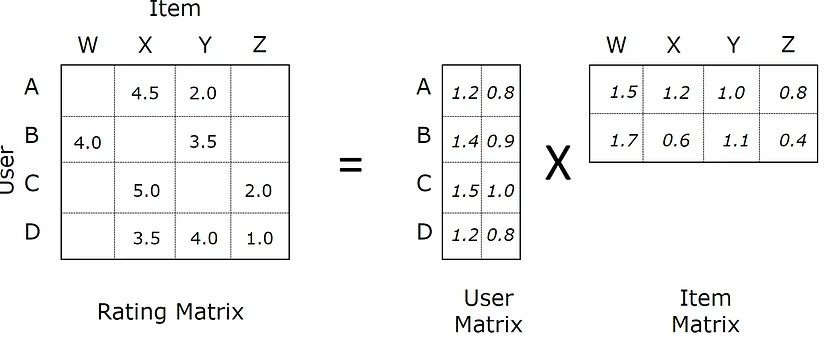
\includegraphics[scale=0.4]{Image1}
	\caption{La factorisation de matrice. Source\footcite{ghosh2018matrixfactorization}}
\end{figure}
~

L'algorithme pourra ensuite utiliser ces scores afin de recommander du contenu inconnu à l'utilisateur sur base de ces prédictions.
Cette méthode de factorisation des matrices permet d'exploiter les données existantes afin de proposer des recommandations de contenu inconnu aux utilisateurs sur base de ce qu'ils aiment.


\subsubsection{Les algorithmes basés sur le filtrage collaboratif (CF)}
~

Les algorithmes de filtrage collaboratif, ou \textit{collaborative filtering algorithms} sont des algorithmes qui recommandent du contenu à un utilisateur en se basant sur les préférences similaires d'un autre utilisateur\footcite{Oufaida2008}. Il existe ici encore deux types de fonctionnement à ces algorithmes. Il y a ceux basés sur la mémoire et ceux basés sur le modèle.
\begin{enumerate}[(A)]
	\item Algorithme basé sur la mémoire

Les algorithmes basés sur la mémoire utilisent pour leur recommandation des données disponibles directement afin d'identifier des similarités entre des utilisateurs ou du contenu. 
Cette fois-ci encore, les données seront représentées sous forme de matrice utilisateur/contenu. Cette matrice reprenant plusieurs utilisateurs et plusieurs contenus sera ensuite parcourue afin de souligner les données intéressantes à utiliser pour la recommandation. Ici encore, nous pouvons retrouver deux types de filtrage différents\footcite{ibm_recommendation_engine}. Celui basé sur l'utilisateur et celui basé sur le contenu. 

Le premier considère que si des utilisateurs ont les mêmes préférences, ils aimeront le même contenu par la suite et que l'on peut recommander à l'un ce que l'autre a apprécié et pas encore vu.
Le deuxième se penche plutôt sur le comportement des utilisateurs par rapport à un certain contenu. Nous ne regardons pas ici aux caractéristiques du contenu comme dans les algorithmes basés sur le contenu. Nous allons par exemple, regarder si un utilisateur ne regarde des séries que le soir et identifier d'autres utilisateurs qui ne regardent des séries que le soir afin de lui proposer le même contenu.

	\item Algorithme basé sur le modèle
    
Les algorithmes basés sur le modèle utilisent des techniques de \textit{Machine Learning} afin de faire des recommandations\footcite{ibm_recommendation_engine}. Cette méthode se base sur un modèle prédictif afin d'évaluer quel contenu pourrait plaire à l'utilisateur. Ce modèle utilise la matrice utilisateur/contenu comme données d'entrée afin de donner des probabilités sur les préférences futures de l'utilisateur. (Nous verrons dans la partie 2.2 le fonctionnement des modèles de \textit{Machine Learning}.)
Comme pour les algorithmes basés sur le contenu, une méthode de réduction de dimension (comme la factorisation de matrice, expliquée au point 2.1.1) est appliquée à la matrice de base afin d'en extraire deux matrices complètes qui seront utilisées pour les calculs.
\end{enumerate}
\subsubsection{Les algorithmes basés sur des techniques hybrides}
Comme leur nom l'indique, les algorithmes basés sur des techniques hybrides mélangent des techniques d'algorithme basés sur le contenu et sur le filtrage collaboratif. Cela permet de tirer le meilleur des deux approches afin de rendre les recommandations encore plus pertinentes. 
 
 ~\\
Attention ! Il est important de savoir que tous les algorithmes de recommandation n'utilisent pas systématiquement le \textit{Machine Learning}. Néanmoins, la documentation concernant l'algorithme de Spotify le mentionne comme étant un pilier fondamental de son fonctionnement.  

\subsection{Le \textit{Machine Learning (ML)\footcite{Portugal2018}}}
L'apprentissage automatique ou Machine Learning remonte aux années 1950. Le but derrière sa création était de démontrer que "\textit{every aspect of learning or
any other feature of intelligence can in principle be so precisely described that a machine can be made to simulate it}\footcite{mccarthy1955dartmouth}." Les chercheurs voulaient alors simuler le processus d'acquisition de connaissances humaines afin d'améliorer les performances de certaines tâches bien spécifiques grâce à l'expérience acquise. 

Les domaines d'application du \textit{Machine Learning} sont divers. Il peut être utilisé dans le marketing pour cibler des annonces, dans la finance pour des analyses de crédit ou encore dans le milieu du divertissement pour recommander des films ou de la musique.

Il existe plusieurs classifications des méthodes d'apprentissage automatique. Nous allons nous concentrer sur celle-ci.
\subsubsection{L'apprentissage supervisé}

L'apprentissage est dit supervisé lorsque l'on possède les réponses des calculs sur lesquels le modèle s'entraine. Il existe deux types d'apprentissage supervisé. Le premier s'entraine sur des données quantitative et le deuxième s'entraine sur des données qualitatives. 
Un exemple du premier serait un algorithme qui estimerait les coûts de production pour un produit dans une entreprise. Un exemple du deuxième serait un algorithme qui classifierait des mails considérés soit comme spam ou bien non spam. 
	
\subsubsection{L'apprentissage non supervisé}

L'apprentissage est dit non supervisé lorsque l'on ne dispose pas des réponses aux calculs sur lesquels le modèle s'entraine. Il existe ici encore deux types d'apprentissage non supervisé. Le premier visant à segmenter les données afin d'avoir une vue d'ensemble. Le deuxième visant à simplifier des ensembles de données afin de les rendre plus simple à manipuler. 
(comme le modèle prédictif qui aide à prédire les goûts en matière de séries d'une personne sur base des séries qu'elle a déjà vues et qu'elle a appréciées du point 2.1.2.)
	
\subsubsection{L'apprentissage par renforcement}
	
L'apprentissage est dit de renforcement lorsque le modèle expérimente par lui-même et réutilise ces résultats afin d'apprendre en continu. Un exemple serait un modèle qui s'entraine à jouer aux échecs. Le modèle doit ici lui-même générer ses propres données et apprend de son expérience. 

\section{Le cas de Spotify}
Spotify est l'une des plateforme musicale les plus utilisées au monde avec plus de 600 millions d'utilisateurs actifs en 2023\footcite{statista2024spotify}.

La plateforme regroupe un catalogue impressionnant de musiques et de podcasts en tout genre. Il peut être ardu pour les utilisateurs de s'y retrouver et d'explorer cette multitude de choix. C'est pour cela que Spotify s'est muni d'un algorithme intelligent utilisant le \textit{Machine Learning} et ayant pour but de guider les utilisateurs en leur recommandant des chansons qu'ils pourraient aimer. 

Spotify utilise un algorithme de recommandation basé sur des techniques hybrides. Au niveau des algorithmes basés sur le contenu, nous pouvons voir que Spotify analyse les morceaux et en retient les principales caractéristiques telles que l'instrumentation ou le tempo. Il se basera ensuite sur ces caractéristiques afin d'effectuer ses recommandations. Par exemple, si un utilisateur aime et écoute régulièrement des chansons de type Nu Metal avec des voix agressives, des percussions très présentes et des rythmes rapides, Spotify pourra analyser les chansons reprenant les mêmes caractéristiques et les catégorisée de la sorte. Il sera ensuite facile de les recommander. Un utilisateur écoutant régulièrement le groupe System of a Down se verra recommander des artistes faisant le même genre de musique, tel que KoRn ou bien Limp Bizkit. 

Ensuite, au niveau des algorithmes basés sur le filtrage collaboratif, Spotify va comparer les utilisateurs et leurs préférences entre eux. Si un utilisateur A et B apprécient tout deux Thundercat, et que l'utilisateur B apprécie aussi fortement Jamiroquai et l'écoute en même temps que Thundercat, Spotify saura qu'il doit recommander Jamiroquai à l'utilisateur A. Le filtrage collaboratif a analysé les habitudes d'écoute des utilisateurs afin de trouver de potentielles affinités et ainsi recommander de nouvelles musiques.

\section{Les tenants et aboutissants \footcite{Adomavicius2005}\footcite{ibm_recommendation_engine}}
L'utilisation du \textit{Machine Learning} dans l'algorithme de recommandation présente de nombreux avantages tels que la personnalisation des recommandations, l'optimisation de l'algorithme et la bonne scalabilité de ces modèles.

Cependant, ces modèles ne sont pas infaillibles et présentent certaines faiblesses. 

\subsection{Les algorithmes de recommandation basés sur le contenu}
~\\
Bien que les algorithmes de recommandation basés sur le contenu soient basés sur différentes approches, ce qui devraient, de prime abord, garantir une certaine diversité, ces derniers pourraient avoir un certain problème dans la représentation des différentes musiques. En effet, si l'algorithme se base uniquement sur le contenu que l'utilisateur aime, il va uniquement recommander le même genre de contenu. L'utilisateur ne se verra pas recommander de nouveau contenu, ce qui est dommage étant donné l'étendue du catalogue de Spotify. De plus, cette approche peut souffrir de ce que l'on appelle le démarrage à froid, qui est le fait que le système dispose de très peu de données venant de l'utilisateur. Il est donc compliqué de se baser sur peu de contenu afin de proposer des recommandations pertinentes.

\subsection{Les algorithmes de recommandation basés sur le filtrage collaboratif\footcite{patissier2024recommandation}}
~\\
 Les algorithmes de recommandation basés sur le filtrage collaboratif souffrent du même problème. Malgré, ses différentes approches, des problèmes se présentent quand même. Le problème du démarrage à froid est d'autant plus présent ici vu que l'on se base sur les relations entre les différents utilisateurs. Cette méthode sera donc moins performante sur un nouvel utilisateur. Bien que ce système dispose d'une bonne scalabilité pour le moment, qu'en est-il de son application à des environnements reprenant beaucoup plus de données que Spotify ? Les calculs peuvent très vite devenir coûteux en temps et en ressources. 
 
\subsection{Les approches hybrides}
~\\
 Les approches hybrides ont été créés pour pallier les problèmes énoncés ci-dessus. Cependant, certains problèmes surviennent également ici. Tout d'abord, le mélange des différentes techniques peut être difficile à mettre en place et peut être complexe à maintenir à jour. Cette approche nécessite une forte puissance de calcul et une mise en place complexe. Le coût de ces derniers est d'ailleurs d'autant élevé.
\section{Conclusion}
Les algorithmes de recommandation jouent un rôle essentiel dans notre société numérique en aidant les utilisateurs à s'orienter parmi une multitude d'options. Les algorithmes basés sur le contenu se basent sur les préférences des utilisateurs pour prédire leurs préférences futures, bien qu'ils puissent souffrir de problèmes de manque de diversité et de démarrage à froid. Les algorithmes de filtrage collaboratif, quant à eux, utilisent les préférences d'autres utilisateurs similaires pour faire des suggestions, mais ils rencontrent aussi des difficultés telles que le démarrage à froid et la scalabilité. Les approches hybrides, qui combinent les deux méthodes, visent à améliorer la précision des recommandations, mais elles peuvent être complexes à mettre en place et nécessiter des ressources de calcul importantes.

~\\
 L'utilisation du \textit{Machine Learning} dans ces algorithmes, comme le montre le cas de Spotify, permet d'optimiser les recommandations et d'offrir une expérience utilisateur personnalisée. Cependant, il est important de reconnaitre les limites et les défis de liés à chaque approche pour améliorer ces systèmes et proposer des recommandations toujours plus pertinentes et diversifiées. 
\newpage
\printbibliography
\end{document}


